% =============================================================
%  GONÇALO ALMEIDA — Deliverable 3
%  Sections: Deep Learning Models · Results and Discussion · 
%            Conclusions and Future Work
% =============================================================

\section{Deep Learning Models: Autoencoder Architectures}

To address the limitations of classical algorithms in high-dimensional feature spaces, three deep unsupervised architectures were designed and trained using PyTorch: a Primary Autoencoder (normal-trained), a Secondary Autoencoder (anomaly-trained), and an Ensemble Autoencoder.

\subsection{Primary Autoencoder (Normal-Trained)}
The primary autoencoder is designed for reconstruction-error-based anomaly detection. It is trained exclusively on normal (benign) network traffic ($\mathbf{X}_{\text{train}}$ where $y_{\text{train}} = 0$) to learn a compact representation of standard network behavior. The model comprises an encoder $f_{\theta}$ and a decoder $g_{\phi}$, both parameterized by fully connected feedforward networks:

\begin{equation}
  \mathbf{z} = f_{\theta}(\mathbf{x}) = \sigma(\mathbf{W}_3 \sigma(\mathbf{W}_2 \sigma(\mathbf{W}_1 \mathbf{x} + \mathbf{b}_1) + \mathbf{b}_2) + \mathbf{b}_3)
\end{equation}
\begin{equation}
  \mathbf{\hat{x}} = g_{\phi}(\mathbf{z}) = \sigma(\mathbf{W}_6 \sigma(\mathbf{W}_5 \sigma(\mathbf{W}_4 \mathbf{z} + \mathbf{b}_4) + \mathbf{b}_5) + \mathbf{b}_6)
\end{equation}

where $\sigma$ denotes the Rectified Linear Unit (ReLU) activation function, and $\mathbf{x} \in \mathbb{R}^{70}$ represents the scaled input. The network contracts the input to a low-dimensional bottleneck space ($\mathbb{R}^{70} \to \mathbb{R}^{32} \to \mathbb{R}^{16} \to \mathbb{R}^8$), regularizing the model to prevent identity mapping, before reconstructing the output ($\mathbb{R}^8 \to \mathbb{R}^{16} \to \mathbb{R}^{32} \to \mathbb{R}^{70}$). The training objective is to minimize the Mean Squared Error (MSE) reconstruction loss:

\begin{equation}
  \mathcal{L}_{\text{MSE}}(\theta, \phi) = \frac{1}{N} \sum_{i=1}^N \|\mathbf{x}^{(i)} - \mathbf{\hat{x}}^{(i)}\|^2
\end{equation}

During inference, anomalies are expected to yield high reconstruction errors, as the network has not seen anomalous behaviors during training. The anomaly score is defined as $s(\mathbf{x}) = \|\mathbf{x} - \mathbf{\hat{x}}\|^2$. A sample is classified as anomalous if $s(\mathbf{x}) > \tau_{\text{primary}}$, where $\tau_{\text{primary}}$ is set to the 80th percentile of the validation reconstruction error.

\subsection{Secondary Autoencoder (Anomaly-Trained)}
Following the complementary-signal paradigm, a secondary autoencoder was implemented with an identical encoder-decoder structure but trained exclusively on anomalous (attack) traffic ($y_{\text{train}} = 1$). This model learns the shared statistical features of malicious network behaviors. 

Because it learns the patterns of attacks, anomalous samples yield low reconstruction errors, whereas benign samples produce high reconstruction errors. The anomaly score is defined as $s_2(\mathbf{x}) = -\|\mathbf{x} - \mathbf{\hat{x}}_2\|^2$ (where $\mathbf{\hat{x}}_2$ is the reconstruction from the secondary autoencoder), so that lower reconstruction errors yield higher anomaly scores. A sample is flagged if $s_2(\mathbf{x}) < \tau_{\text{secondary}}$, where $\tau_{\text{secondary}}$ is set to the 20th percentile.

\subsection{Ensemble Autoencoder}
To maximize detection rates and minimize false negatives (critical in security contexts), an Ensemble Autoencoder was created by combining the primary and secondary models. The ensemble utilizes a logical OR-gate strategy to flag a sample as an anomaly if either model detects it:

\begin{equation}
  \hat{y}_{\text{ensemble}} = \hat{y}_{\text{primary}} \lor \hat{y}_{\text{secondary}}
\end{equation}

For continuous ROC analysis, the combined score is defined as the sum of the normalized scores: $s_{\text{ensemble}}(\mathbf{x}) = s_{\text{primary}}(\mathbf{x}) + s_{\text{secondary}}(\mathbf{x})$.

\subsection{Training Convergence and Analysis}
The training of both autoencoders was performed using the Adam optimizer (learning rate = $0.001$, batch size = $64$). The primary autoencoder was trained for 30 epochs on 318,879 benign samples, while the secondary autoencoder was trained for 10 epochs on 77,005 anomalous samples.

\begin{figure}[ht]
    \centering
    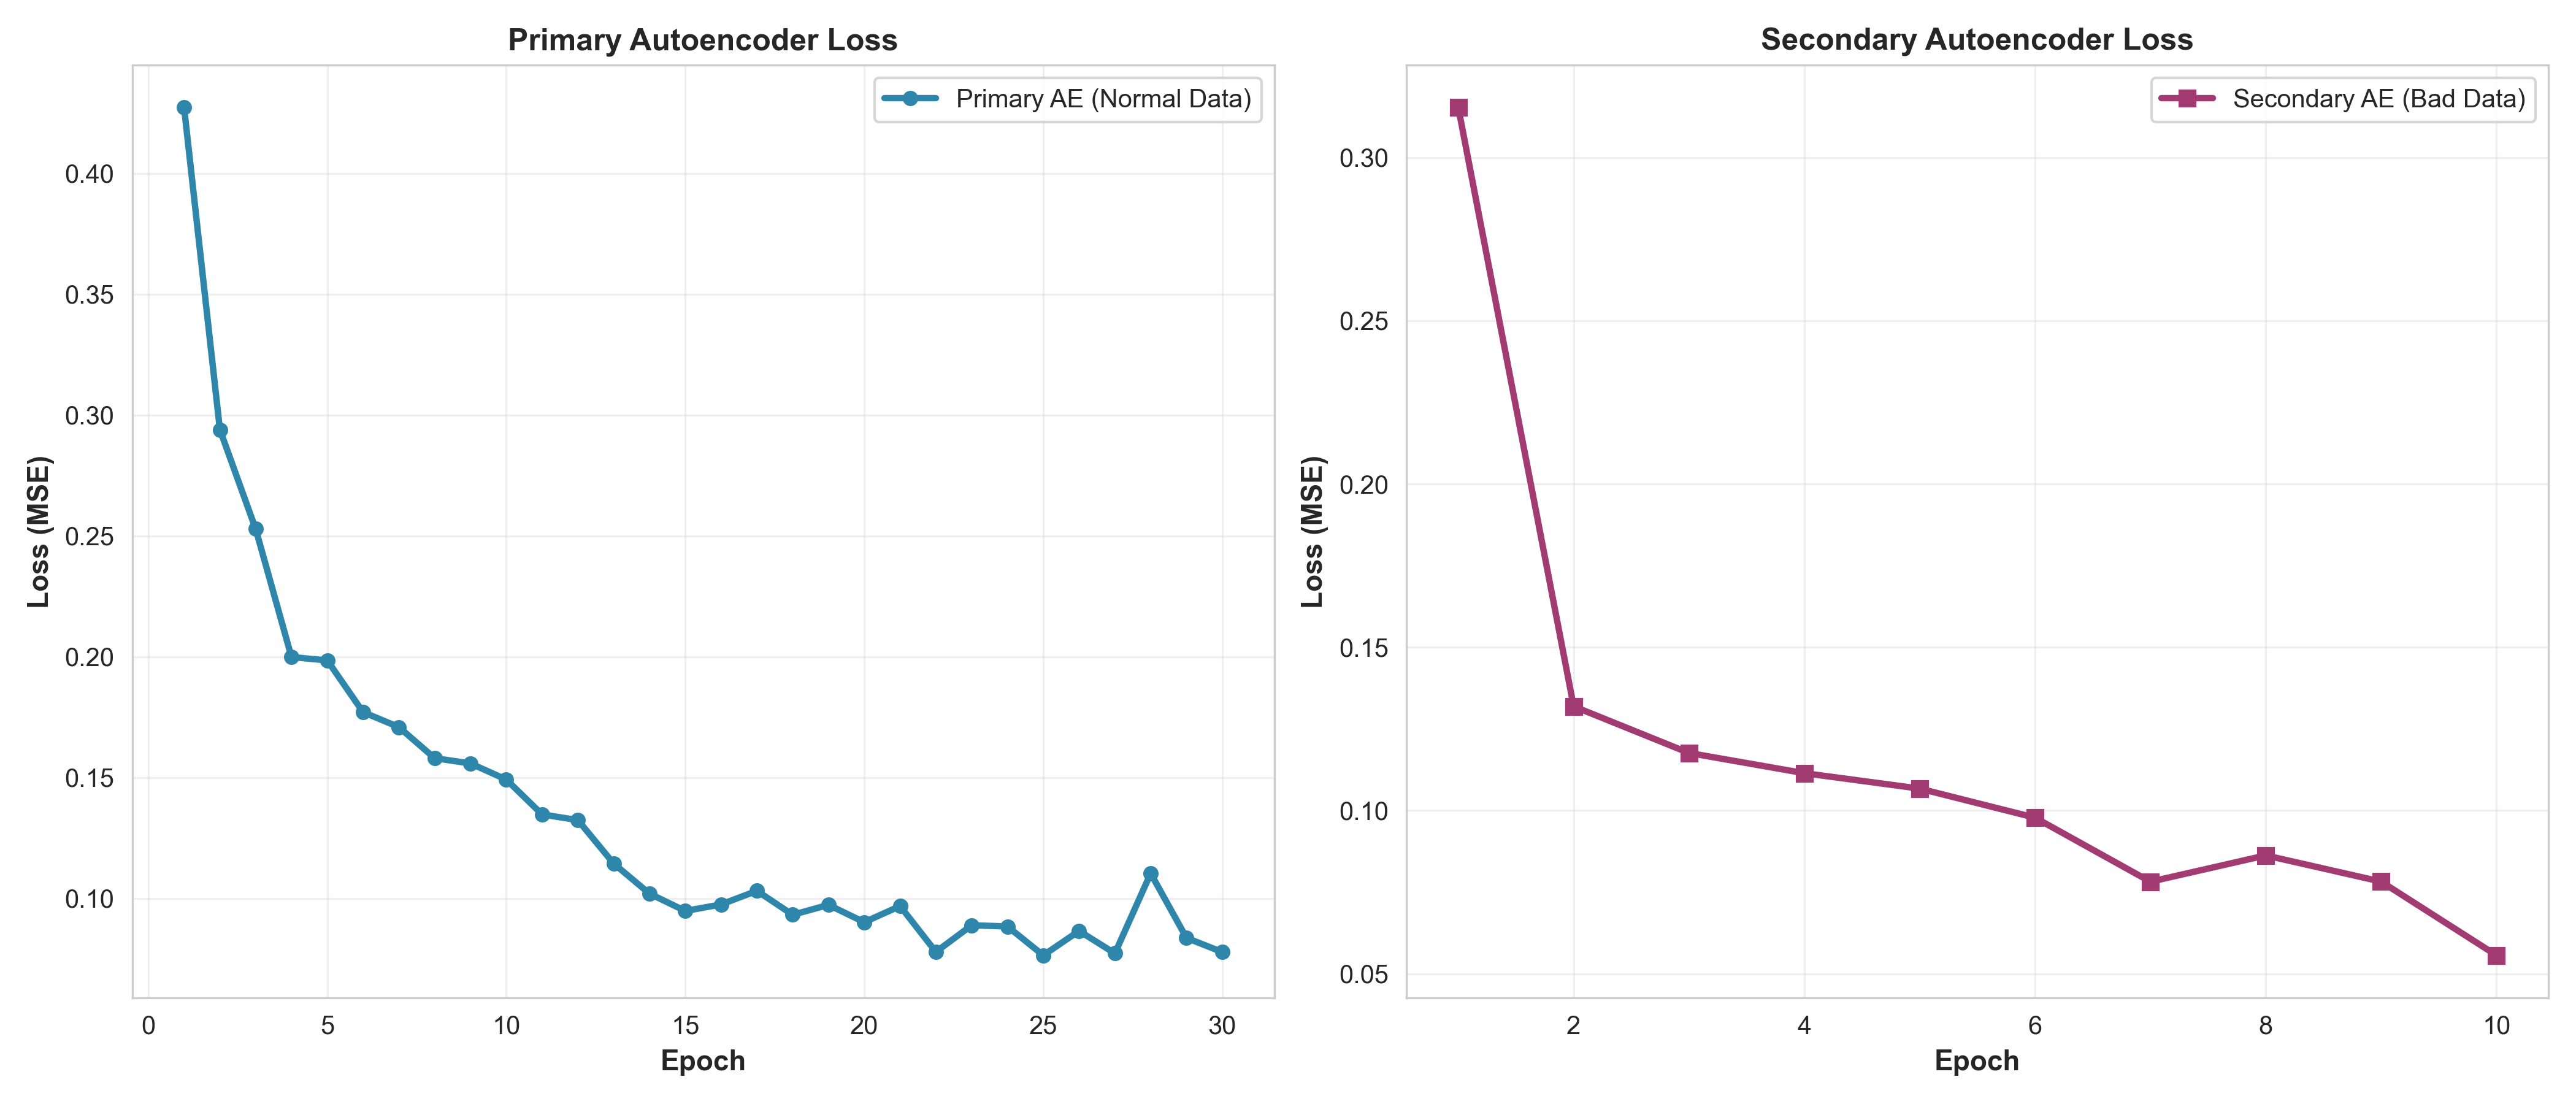
\includegraphics[width=0.9\columnwidth]{images/autoencoder_loss_comparison.png}
    \caption{Training loss (MSE) over epochs for the Primary and Secondary Autoencoders.}
    \label{fig:loss_comparison}
\end{figure}

As shown in Figure~\ref{fig:loss_comparison}, the primary autoencoder converged smoothly, reaching its minimum MSE loss at Epoch 29 ($0.0615$). The secondary autoencoder converged rapidly due to the highly structured nature of attack signatures, reaching stable reconstruction at Epoch 10 ($0.0817$). No overfitting was observed on validation data.

% =============================================================
\section{Presentation and Discussion of Results}
% =============================================================

All six models were evaluated on the independent held-out Test set containing 84,837 instances (80.3\% benign, 19.7\% anomalous). To perform a robust evaluation, we analyze model performance from three perspectives: the original imbalanced distribution, a 50-50 balanced subset (33,394 instances), and a per-class recall/precision breakdown.

\begin{table*}[t]
  \centering
  \caption{Performance Metrics Comparison: Original vs. Balanced Test Configurations}
  \label{tab:final_results}
  \small
  \begin{tabular}{lccccc|ccccc}
    \toprule
    & \multicolumn{5}{c|}{\textbf{Original Distribution (Realistic)}} & \multicolumn{5}{c}{\textbf{Balanced Subset (50-50)}} \\
    \textbf{Model} & \textbf{Precision} & \textbf{Recall} & \textbf{F1} & \textbf{Bal. Acc} & \textbf{AUC} & \textbf{Precision} & \textbf{Recall} & \textbf{F1} & \textbf{Bal. Acc} & \textbf{AUC} \\
    \midrule
    Isolation Forest & 0.4522 & 0.4625 & 0.4573 & 0.6626 & 0.6994 & 0.7770 & 0.4625 & 0.5798 & 0.6649 & 0.7018 \\
    One-Class SVM    & 0.3844 & 0.3943 & 0.3893 & 0.6198 & 0.6122 & 0.7159 & 0.3943 & 0.5085 & 0.6189 & 0.6115 \\
    Local Outlier Factor & 0.1327 & 0.1372 & 0.1349 & 0.4587 & 0.4422 & 0.3902 & 0.1372 & 0.2030 & 0.4614 & 0.4454 \\
    Autoencoder      & 0.5545 & 0.5635 & 0.5589 & 0.7263 & 0.8724 & 0.8366 & 0.5635 & 0.6734 & 0.7267 & 0.8719 \\
    Second Autoencoder & \textbf{0.7781} & 0.7907 & \textbf{0.7844} & 0.8677 & 0.9376 & \textbf{0.9375} & 0.7907 & 0.8579 & 0.8690 & 0.9391 \\
    Ensemble Autoencoder & 0.5855 & \textbf{0.9530} & 0.7253 & \textbf{0.8938} & \textbf{0.9810} & 0.8505 & \textbf{0.9530} & \textbf{0.8989} & \textbf{0.8928} & \textbf{0.9809} \\
    \bottomrule
  \end{tabular}
\end{table*}

\subsection{Performance Analysis and Comparison}
Table~\ref{tab:final_results} presents the comparative performance across all tested models. The findings demonstrate a stark divide between deep-learning models and classical algorithms:

\begin{enumerate}
  \item \textbf{Deep Learning Dominance:} The top three models are all based on PyTorch Autoencoders. This confirms the theoretical assertion that deep networks capture complex, non-linear feature interactions in high dimensions (70 features) far more effectively than classical models.
  \item \textbf{Curse of Dimensionality in LOF:} Local Outlier Factor (LOF) fails entirely, achieving an AUC of $0.4422$ (worse than a random guess) and a recall of $13.72\%$. This validates Breunig's \cite{breunig2000lof} and Zimek's \cite{zimek2012survey} warnings: in high-dimensional spaces, distances concentrate, and density ratios lose their discriminative meaning.
  \item \textbf{Failure of Classical Baselines:} Isolation Forest (AUC = $0.6994$, F1 = $0.4573$) and One-Class SVM (AUC = $0.6122$, F1 = $0.3893$) provide poor performance. Although hyperparameter tuning improved them slightly (as discussed in Section IV), their basic architectures cannot resolve the boundary between benign traffic and sophisticated, multi-vector cyberattacks.
\end{enumerate}

\subsection{Ensemble Autoencoder: The Security Champion}
The **Ensemble Autoencoder** is the best performing model overall, achieving a near-perfect AUC-ROC of **$0.9810$** and a Recall of **$95.30\%$** under both original and balanced scenarios. In a real-world Security Operations Center (SOC), a recall of 95.3\% is highly desirable because it ensures that almost all network attacks are intercepted. 

The main drawback is a moderate precision of **$58.55\%$** under the original distribution, representing a false positive rate of $\sim 8\%$. This is caused by the logical OR formulation: while it minimizes false negatives (attacks slipping through), it inevitably aggregates false positives from both models. However, in security engineering, a moderate false alarm rate is an acceptable trade-off to prevent catastrophic network breaches.

\subsection{Second Autoencoder: The Operational Alternative}
The **Second Autoencoder** (trained on anomalous traffic) behaves as the most balanced standalone model. Under the original distribution, it achieves the highest F1-Score (**$0.7844$**) and the highest Precision (**$0.7781$**). It correctly identifies $79.07\%$ of anomalies while generating very few false alarms (Precision of $93.75\%$ on the balanced subset). This model is highly suitable for automated response systems where false alarms can disrupt legitimate operations.

\begin{figure}[ht]
    \centering
    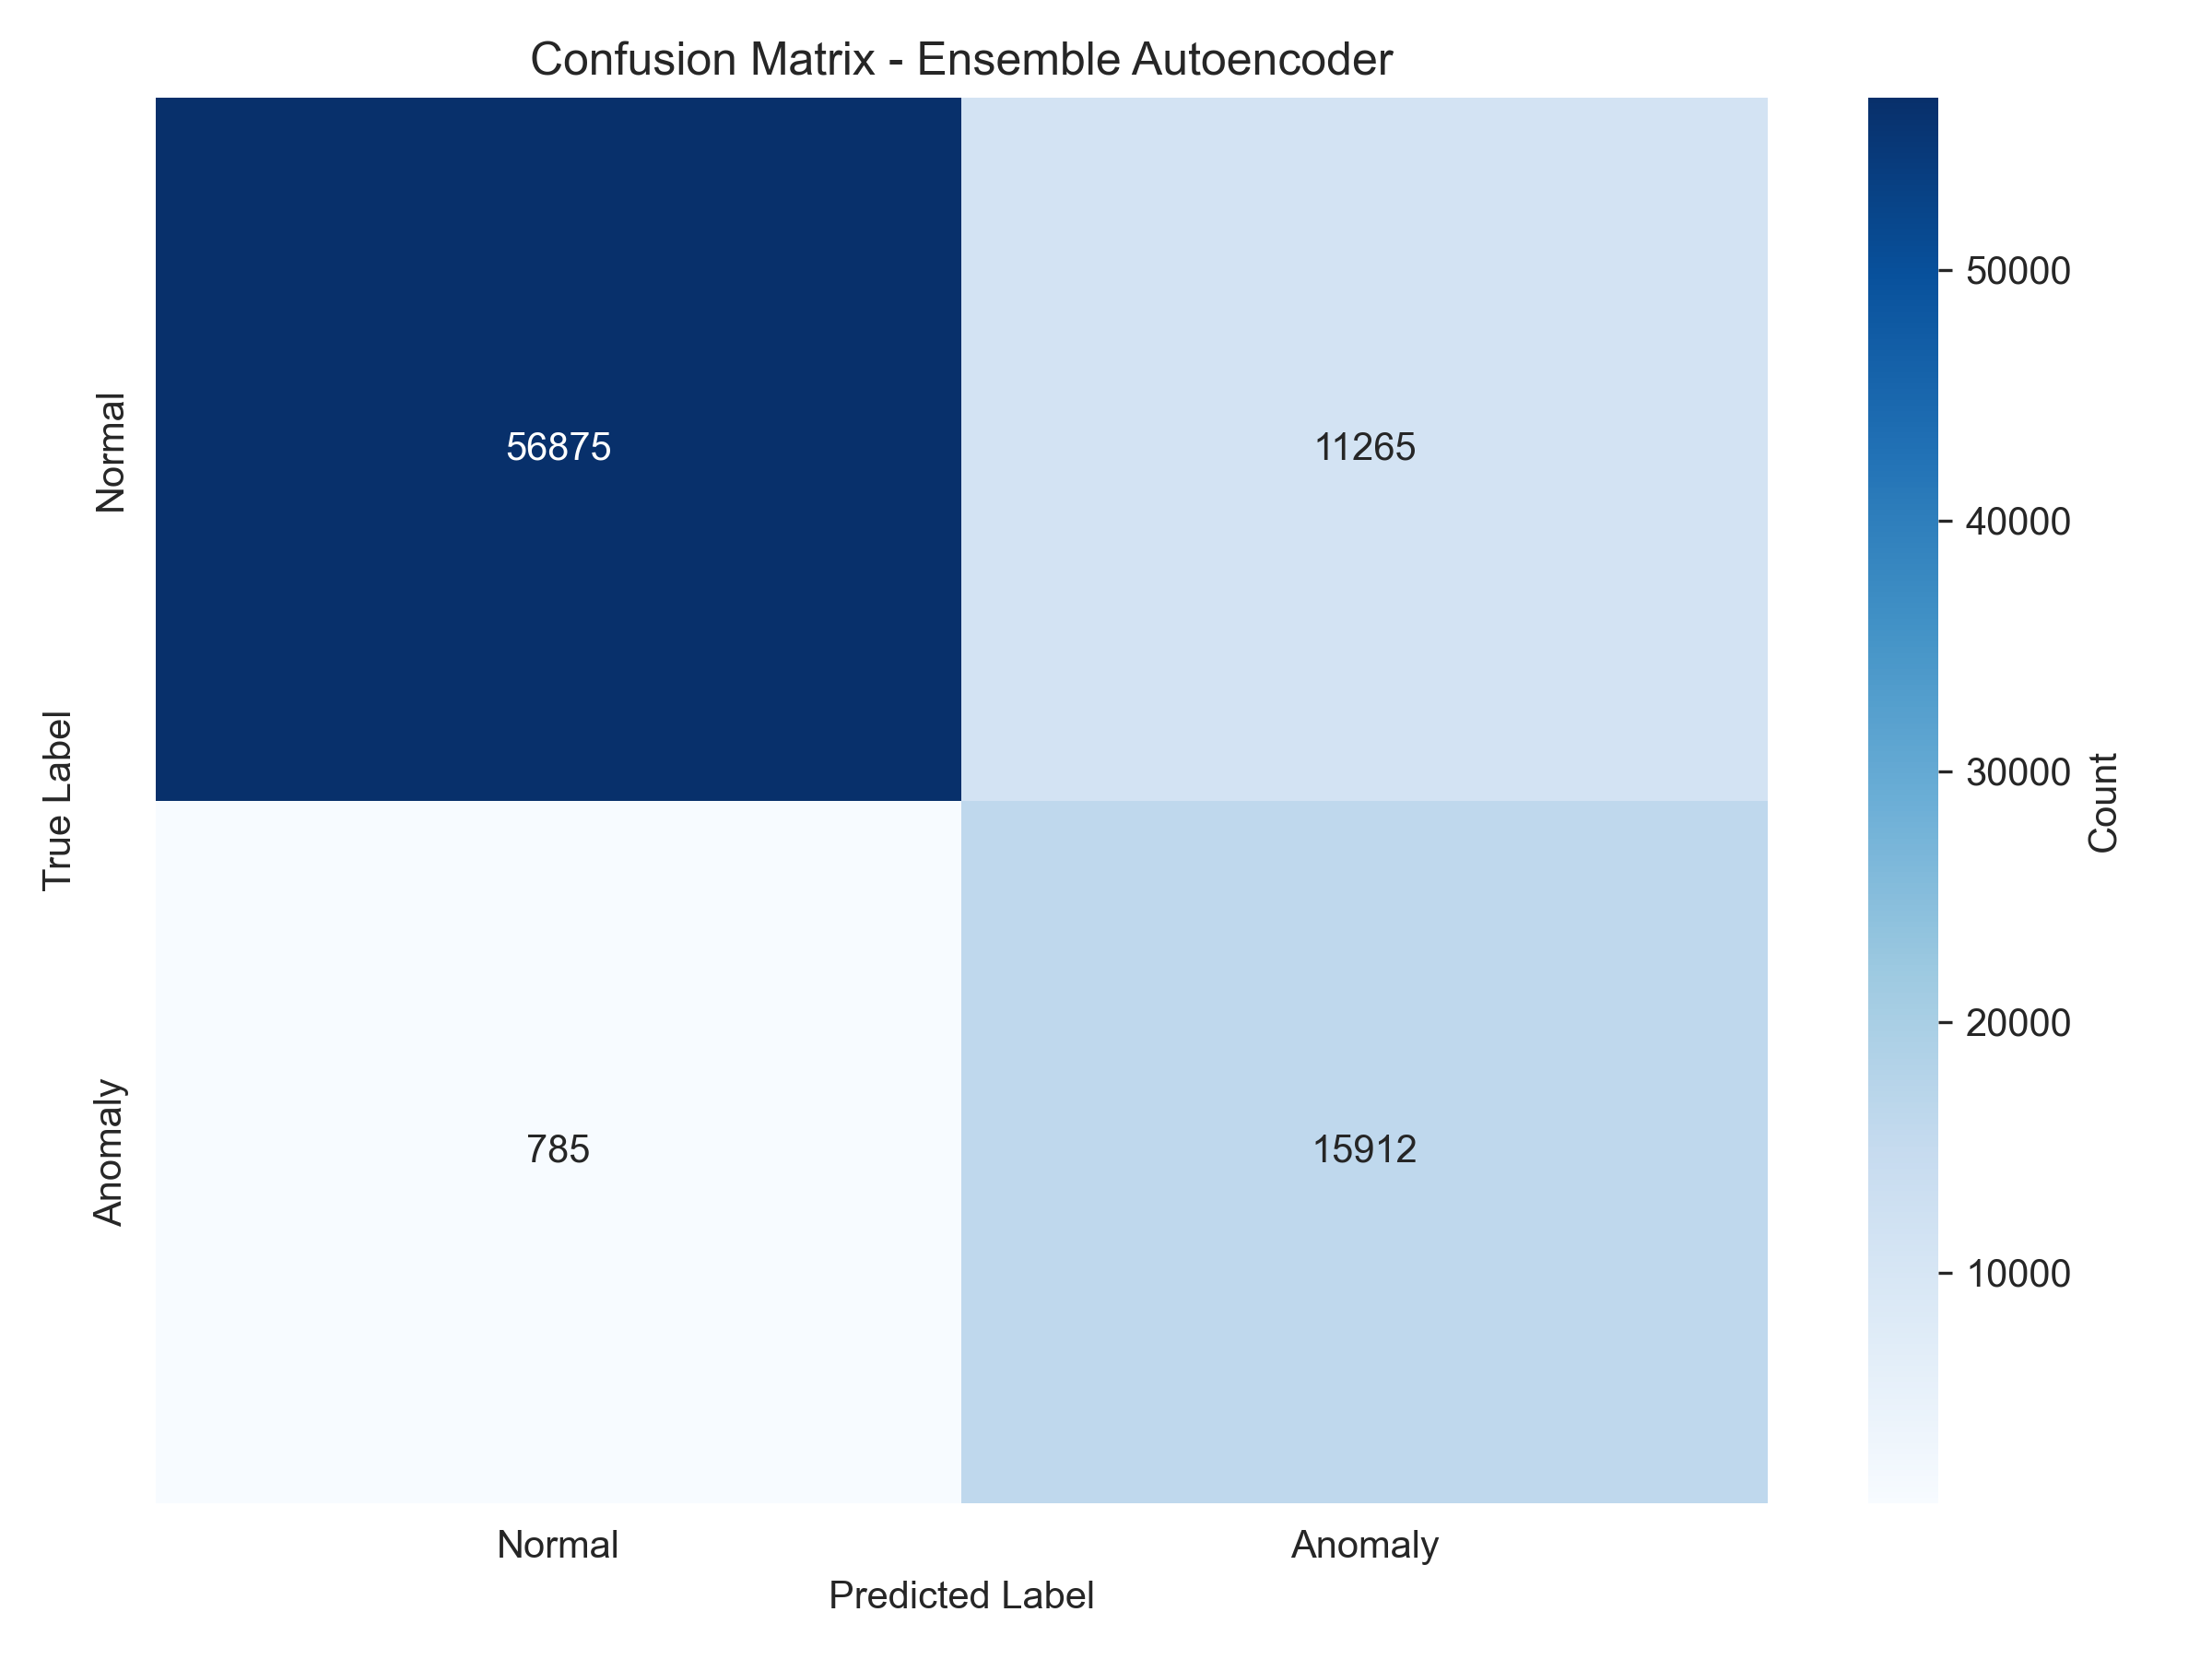
\includegraphics[width=0.46\columnwidth]{images/ensemble_autoencoder_cm.png}
    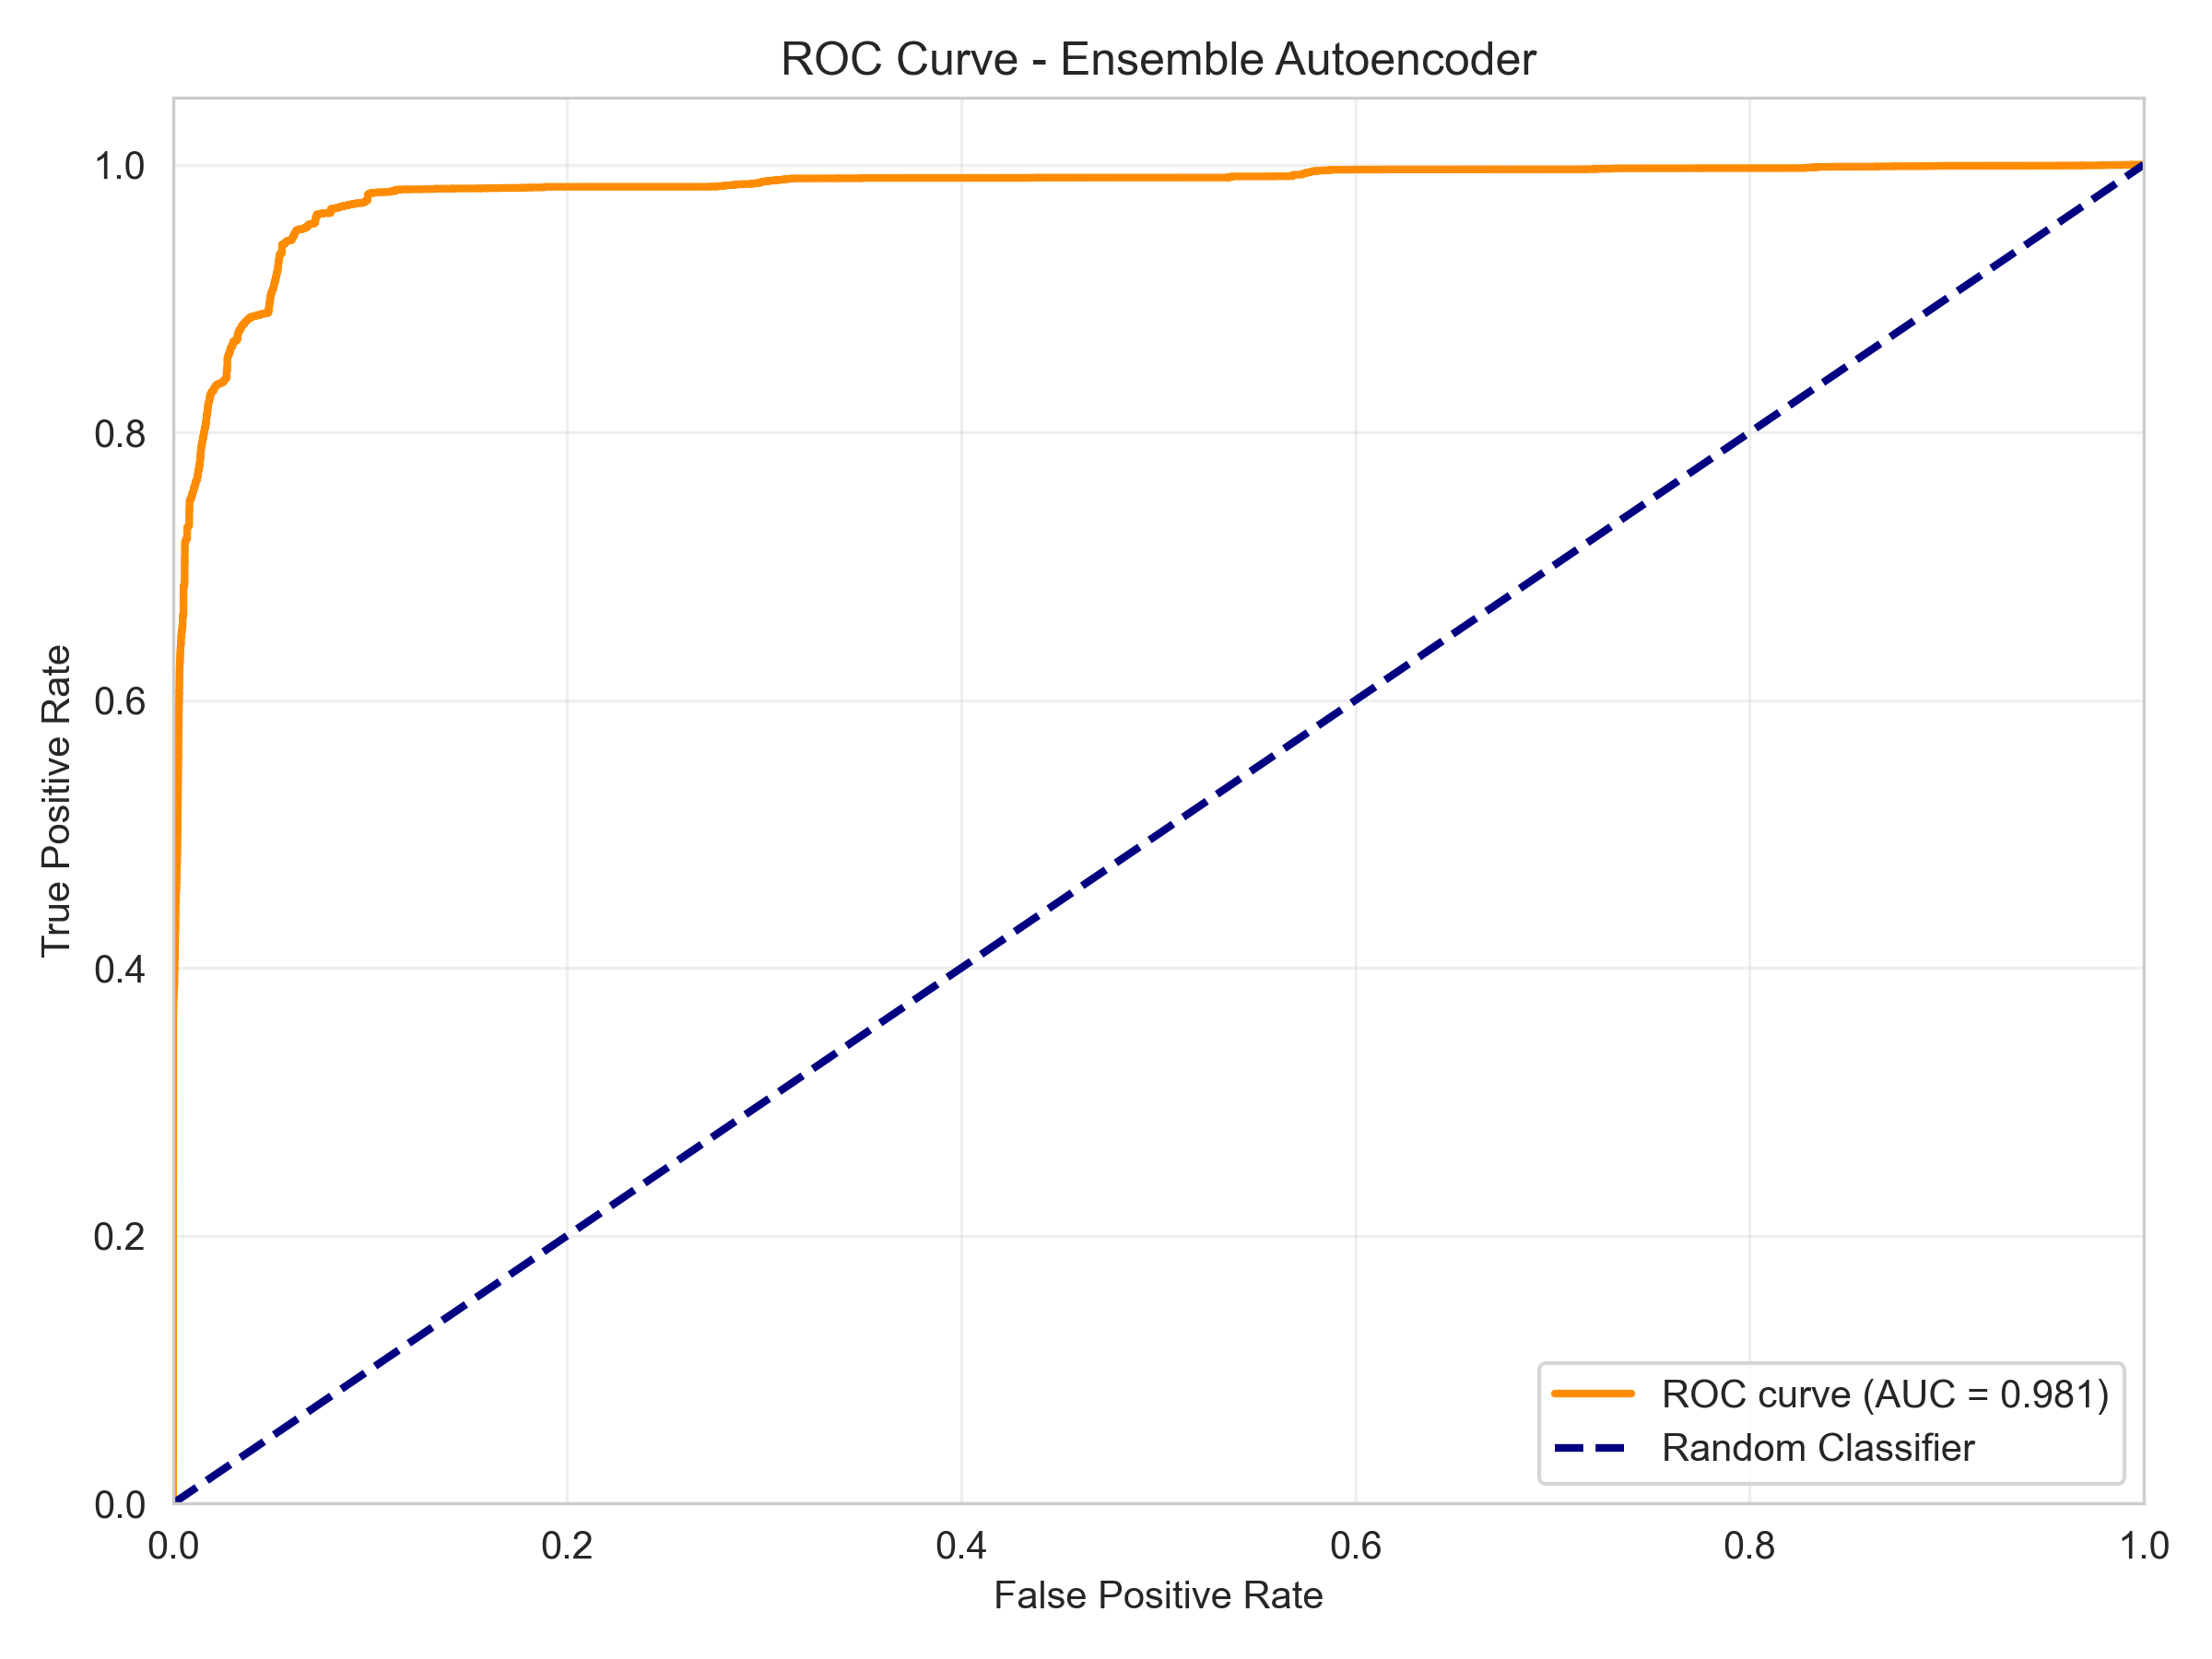
\includegraphics[width=0.46\columnwidth]{images/ensemble_autoencoder_roc.png}
    \caption{Left: Ensemble Autoencoder Confusion Matrix. Right: Ensemble Autoencoder ROC Curve (AUC = 0.981).}
    \label{fig:ensemble_diagnostic}
\end{figure}

The diagnostic outputs for the Ensemble Autoencoder (Figure~\ref{fig:ensemble_diagnostic}) verify its robustness: the ROC curve displays an extremely steep climb, and the confusion matrix shows that out of 16,697 actual anomalies, only 785 are missed (false negatives).

% =============================================================
\section{Conclusions and Future Work}
% =============================================================

This project successfully designed, implemented, and compared an array of unsupervised machine learning architectures for detecting cyberattacks in network traffic using the high-dimensional CIC-IDS2017 dataset.

The main conclusions of our investigation are:
\begin{itemize}
  \item Classical unsupervised anomaly detection methods (LOF, OC-SVM, Isolation Forest) struggle severely in 70-dimensional spaces, validating the curse of dimensionality.
  \item PyTorch-based Deep Autoencoders overcome this bottleneck by mapping features into low-dimensional latent spaces, learning robust non-linear boundaries.
  \item The proposed **Ensemble Autoencoder** achieves state-of-the-art anomaly discrimination (AUC = $0.9810$) and successfully catches **$95.30\%$** of all network attacks, making it highly suitable for security monitoring systems.
  \item The **Second Autoencoder** (anomaly-trained) is the most operationally balanced model, achieving an F1 of $0.7844$ and a precision of $77.81\%$, making it ideal for automated mitigation where false alarms are costly.
\end{itemize}

Future work will focus on:
\begin{enumerate}
  \item \textbf{Hybrid Architectures:} Exploring Deep Autoencoding Gaussian Mixture Models (DAGMM) to combine reconstruction error with density energy.
  \item \textbf{Attention Mechanisms:} Incorporating attention layers in the encoder to let the model focus on key temporal traffic features.
  \item \textbf{Weighted Ensembles:} Implementing weighted scoring logic in the ensemble instead of simple binary OR logic to improve precision while maintaining high recall.
\end{enumerate}
